\documentclass{article}
\usepackage[utf8]{inputenc}
\usepackage{fancyhdr}
\usepackage{graphicx}
\usepackage{geometry}
\usepackage{float}

% ---- Commands ------- %
\newcommand{\documentNumber}[1]{
    \LARGE  \textbf{ Processrapport }
    \\
    \medskip
}
\newcommand{\documentVersion}[1]{
    \medskip
}
\newcommand{\documentTitle}[1]{
    \centerline{\rule{13cm}{0.4pt}}
    \bigskip \bigskip
    \LARGE \textbf{Projekt IDA3} \\
    \bigskip
    \LARGE {#1} \\
    \bigskip \bigskip
    \centerline{\rule{13cm}{0.4pt}}
}

\newcommand{\documentDate}[1]{
    \date {#1} 
}


\renewcommand{\arraystretch}{1.7}  % Vertical padding for tables

\renewcommand{\contentsname}{Innehållsförtäckning}

% --- Header & Footer ---- %
\pagestyle{fancy}
\lhead{\leftmark}
\rhead{}
\rfoot{\thepage}
\cfoot{}
\lfoot{}


% ------------------------------------------------ #

% ----- FILL THIS ----- %
\title {
    \documentNumber {01}    

    % Full name - SHORTNAME
    \documentTitle {Helsingborg Event and Convention Bureau}
    
    % Format: YYYY-MM-DD
    \documentDate {2021-09-29}
    \documentVersion Vv 0.1
    
    \author{Anna Bergvall - Oscar Blixt - Pontus Persson - Filip Sjövall - David Vilppu - Sabah Zafar}
}

\begin{document}
\addtocontents{toc}{\protect\setcounter{tocdepth}{2}}
\maketitle

\thispagestyle{empty}



\newpage

\tableofcontents


\newpage

\section{Dokument Historia}
\begin{tabular}{ l | l | l }
    Version & Date & Description \\
    \hline
    0.1 & 2021-09-29 & Dokumentet skapat. Målbild och process. \\
    \hline
   
\end{tabular}

\newpage
% ----- SKRIV UNDER VARJE TITEL ----- %
\section{Analys}
\subsection{Målbild}
\subsubsection{Elevator Statement}


Vår målgrupp är kommuner och städer som önskar att gå med i det globala nätverket Global
Destination Sustainability Movement (GDSM). Som medlem i nätverket rapporteras det
årligen in hållbarhetsdata som bidrar till en positiv utveckling av staden som en mötes-och
evenemangsdestination. \\ \indent Sustainable Form är ett digitalt rapporteringsverktyg som samlar in
och sammanställer hållbarhetsdata från aktörer inom besöksnäring i städer och kommuner.
Till skillnad från Google Forms ger vår digitala rapporteringsverktyg skräddarsydd
sammanställning och större kontroll över distribution och administration av den insamlade
datan. Sustainable Form kan användas av aktörer med olika tekniska färdigheter eftersom den
är lättanvändbar med simpla funktioner.

\subsubsection{Kravspecifikation och samsyn}

\begin{figure}[htp]
    \centering
    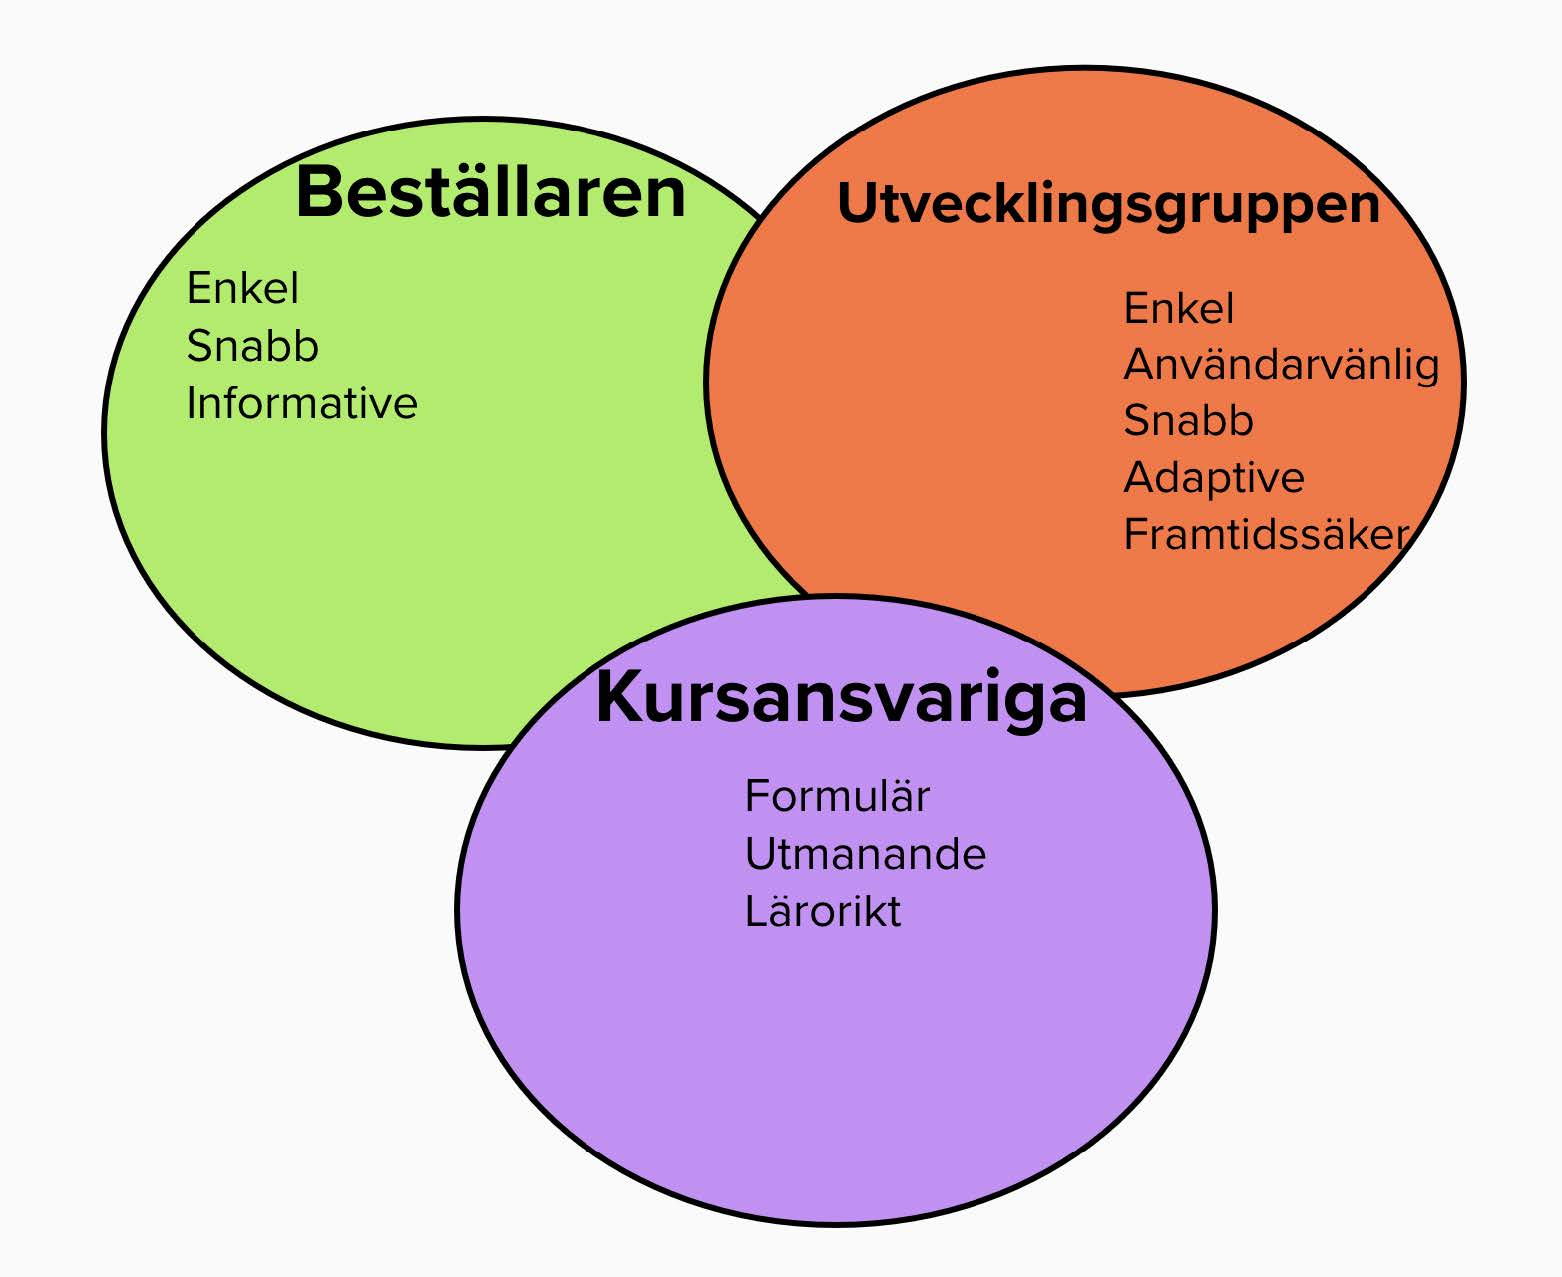
\includegraphics[width = 155px]{malbild.jpg}
    \label{fig:24}
\end{figure}

Hur stabil är målbilden?

\begin{enumerate}
	\item Vårt digitala rapporteringsverktyg är inte helt nyskapande utan det finns liknande
lösningar som exempelvis Google Forms men vår lösning kommer med några unika
funktioner som är skräddarsydda med större kontroll över distribution och
administration. 

	 \item Helsingborg Convention and Event Bureau(HCEB) har erfarenhet av datainsamling
men saknar ett system som kan sammanställa datan. HCEB har således inte
mycket erfarenhet av själva mjukvaruutvecklingen. På grund av deras begränsade kunskap har vi friare händer att bestämma över produkten.

\item I Informationen vi fått från HCEB framgår inte mer än att beställaren vill ha en sammanställning av data som aktörer skickar in. På grund av den begränsade informationen kan vi anta att vi inte kan få en större mängd feedback på själva utvecklingen.

\item Eftersom HCEB är mer intresserade av att det finns ett färdigutvecklat system och
inte några specifika funktioner kommer troligtvis förändringar av utvecklingen att
välkomnas.

\item Kontakten hålls vid förutbestämda handledningstillfällen med jämna mellanrum och
vid behov kommer möten bokas för tydlighetens skull.

\item Tidigare har projektgruppen gjort en liknande utvecklingsprocess och har någorlunda
erfarenhet av utvecklingsarbetet och liknande tekniker.

\item Slutanvändarna har liknande intressen av arbetet och produkten som utvecklas.
\end{enumerate}


\newpage
\subsection{Process}
\subsubsection{WBS}
Då vi fortfarande befinner oss i början av projektet har vi begränsad information. Därför har vi valt att dela arbetet i breda kategorier. På nivå 1 i vår WBS ligger slutprodukten som har givits namnet Sustainable Form. De kategorier på nivå 2 är sådana som vi vet att vi kommer behöva göra: 
\begin{itemize}
\item Databas
\item Grafiskt användargränssnitt, GUI
\item Test
\item Design + Prototyp
\item API
\end{itemize}
\begin{figure}[htp]
    \centering
    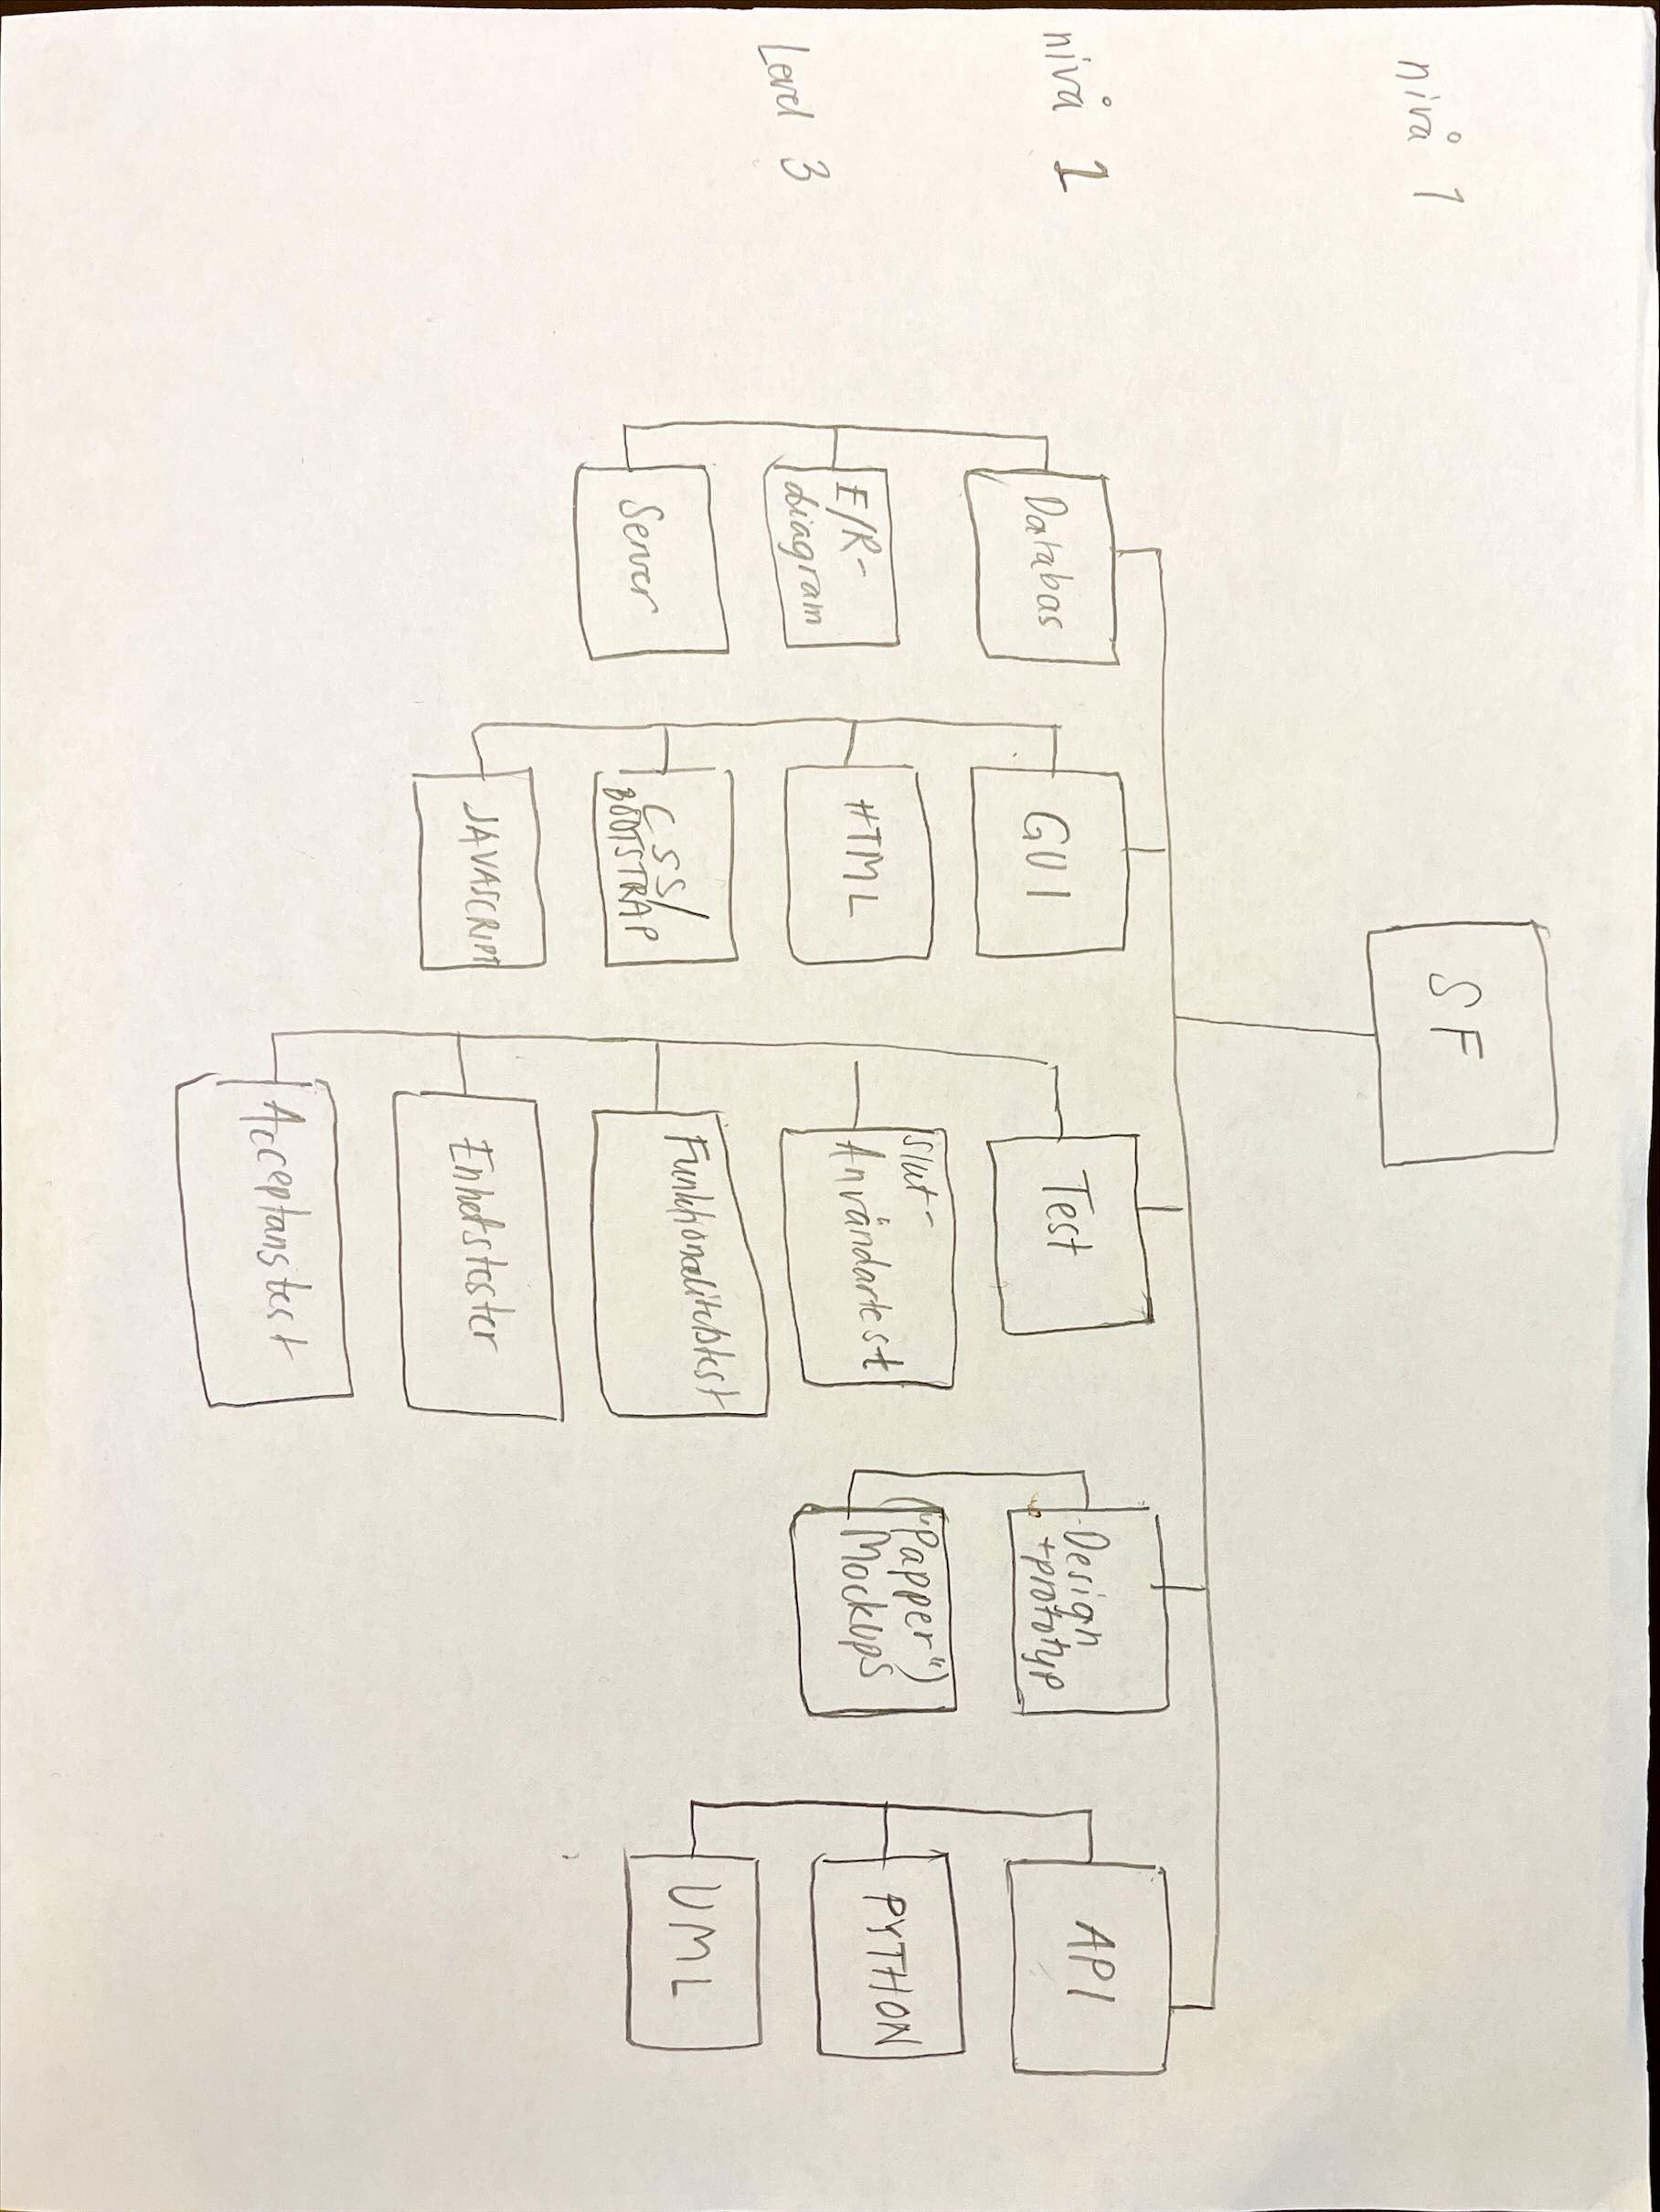
\includegraphics[width = 175px,angle=90]{WBS.jpg}
    \label{fig:24}
\end{figure}

Varje modul delades upp i underuppgifter som sattes in i WBS på nivå 3. Databasen består av arbetsuppgifterna E&/R-diagram och server, GUI:n består av HTML, CSS&/Bootstrap och JavaScript och under testmodulen hittar vi användartest, funktionstest, enhetstester och acceptanstest. Modulen Design&/Prototyp har en underuppgift "paper mockups", dvs att tillverka low fidelity-prototyper, och slutligen så har API som submoduler python och UML. Vi har valt att använda python eftersom ingen i teamet har gjort något projekt i python tidigare och det känns orimligt att ta examen från LTH och inte ha jobbat i det språket.
\subsubsection{PERT}

Det är lite svårt att veta var man ska börja eftersom vi inte har så mycket kunskap om projektet än. Vi tänkte att en design-mockup är ett bra ställe att börja på eftersom det kan involvera kunden tidigt. Dessutom hjälpte PERT oss att se sambanden mellan de olika aktiviteterna. Vi har tvingats att tänka på arbetsbördan på ett mycket konkret sätt. Det blir också tydligt att vissa aktiviteter tar betydligt längre tid än andra.

\newpage
\begin{tabular}{c||c||c||c}
    ID & är beroende av... & Beskrivning av aktivitet/mål & Tidsuppskattning \\
   \hline
    &&& \begin{tabular}{ccc}
         Låg & Mellan & Hög  \\
 
    \end{tabular}
  \\
\hline
  1 & - & Design mockup & \begin{tabular}{ccc}
                            6 h & 12 h & 18 h \\
      
      
                            \end{tabular}
  \\
  \hline
  2 & - & E/R-diagram & \begin{tabular}{ccc}
                         2 h & 3 h & 4 h  \\
       
                        \end{tabular}
  \\
  \hline
    3 & - & GUI & \begin{tabular}{ccc}
                         30 h & 48 h & 60 h  \\
       
                        \end{tabular}
  \\
    \hline
    4 & Databasen och GUI & API & \begin{tabular}{ccc}
                         120 h & 240 h & 480 h  \\
       
                        \end{tabular}
  \\
  
    \hline
    5 & E/R-diagram & Databas & \begin{tabular}{ccc}
                        10 h  & 16 h & 24 h  \\
       
                        \end{tabular}
  \\
  
    \hline
    6 & - & JavaScript & \begin{tabular}{ccc}
                        8 h & 16 h &  24 h \\
       
                        \end{tabular}
  \\
    \hline
    7 & - & UML & \begin{tabular}{ccc}
                         8h & 12 h & 16 h  \\
       
                        \end{tabular}
  \\
    \hline
    8 & - & Användartest & \begin{tabular}{ccc}
                         4 h & 8 h & 12 h  \\
       
                        \end{tabular}
  \\
    \hline
    9 & - & Funktionstest & \begin{tabular}{ccc}
                         60 h & 120 h & 240 h  \\
       
                        \end{tabular}
  \\
    \hline
    10 & - & Databastest & \begin{tabular}{ccc}
                         24 h & 48 h & 92 h  \\
       
                        \end{tabular}
  \\
  
\end{tabular}

\\
\begin{figure}[htp]
    \centering
    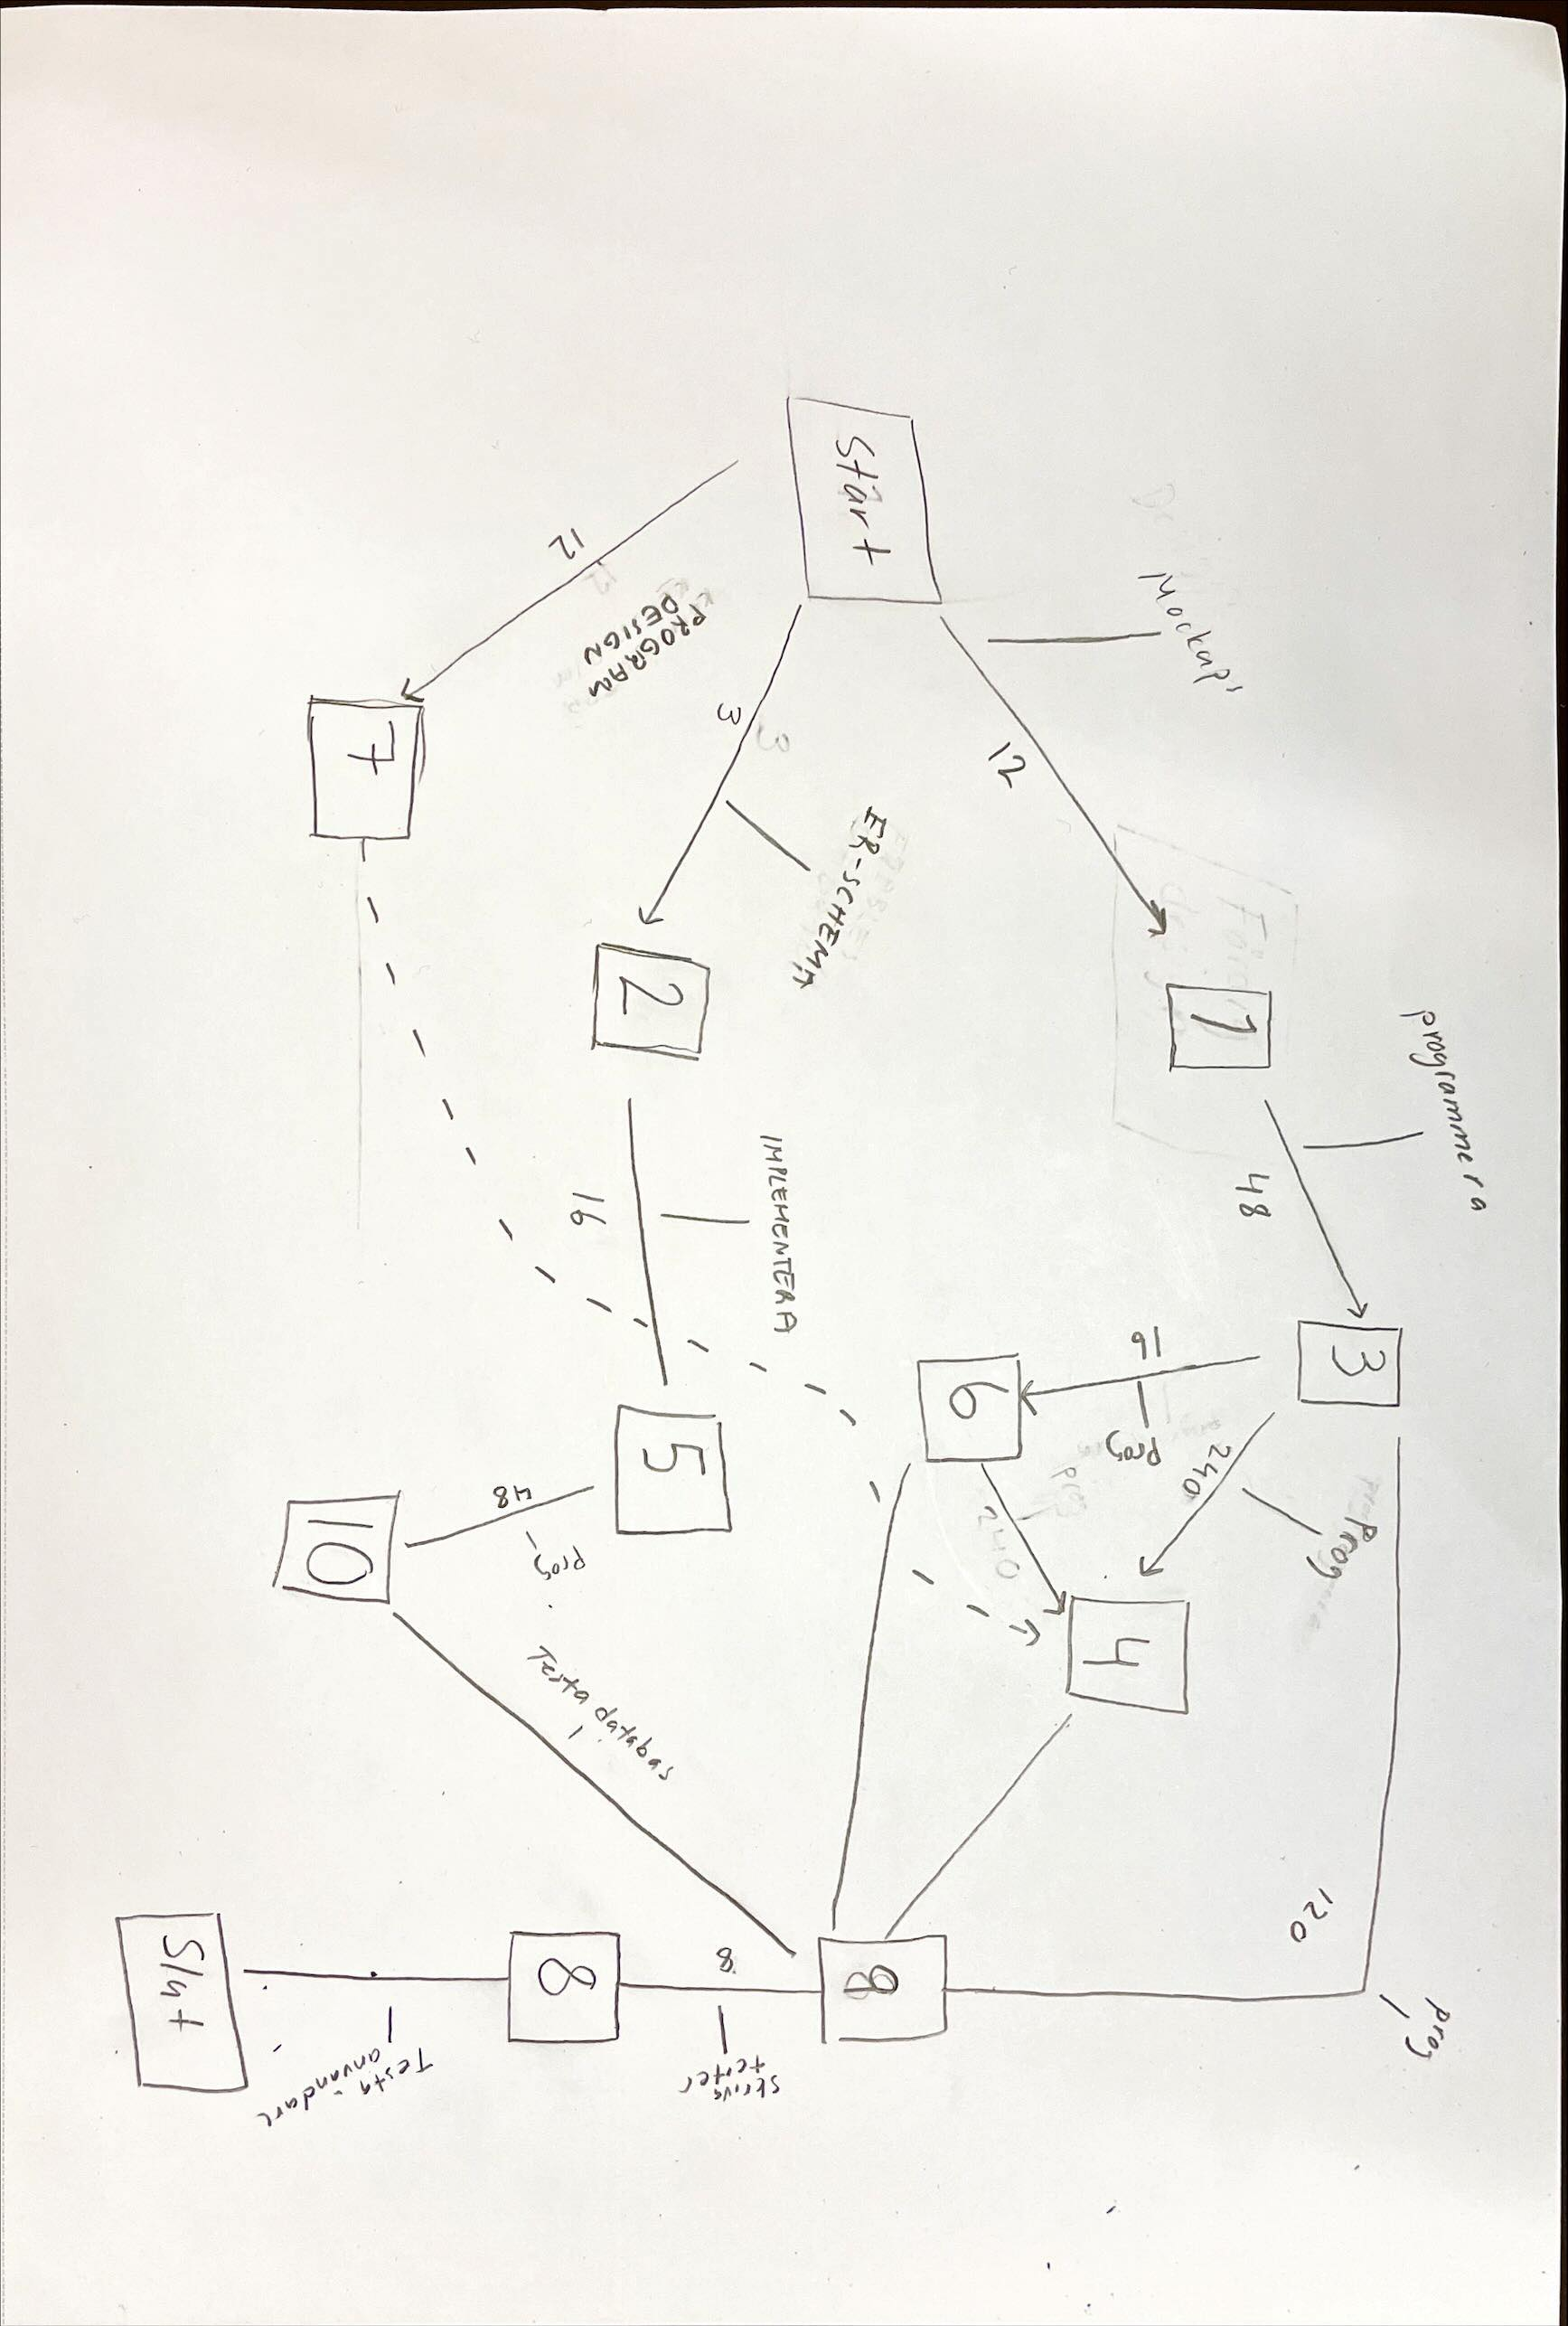
\includegraphics[width = 175px, angle=90]{Pert.jpg}
    \label{fig:24}
\end{figure}

\newpage
\subsubsection{Tidsplan}

\begin{figure}[htp]
    \centering
    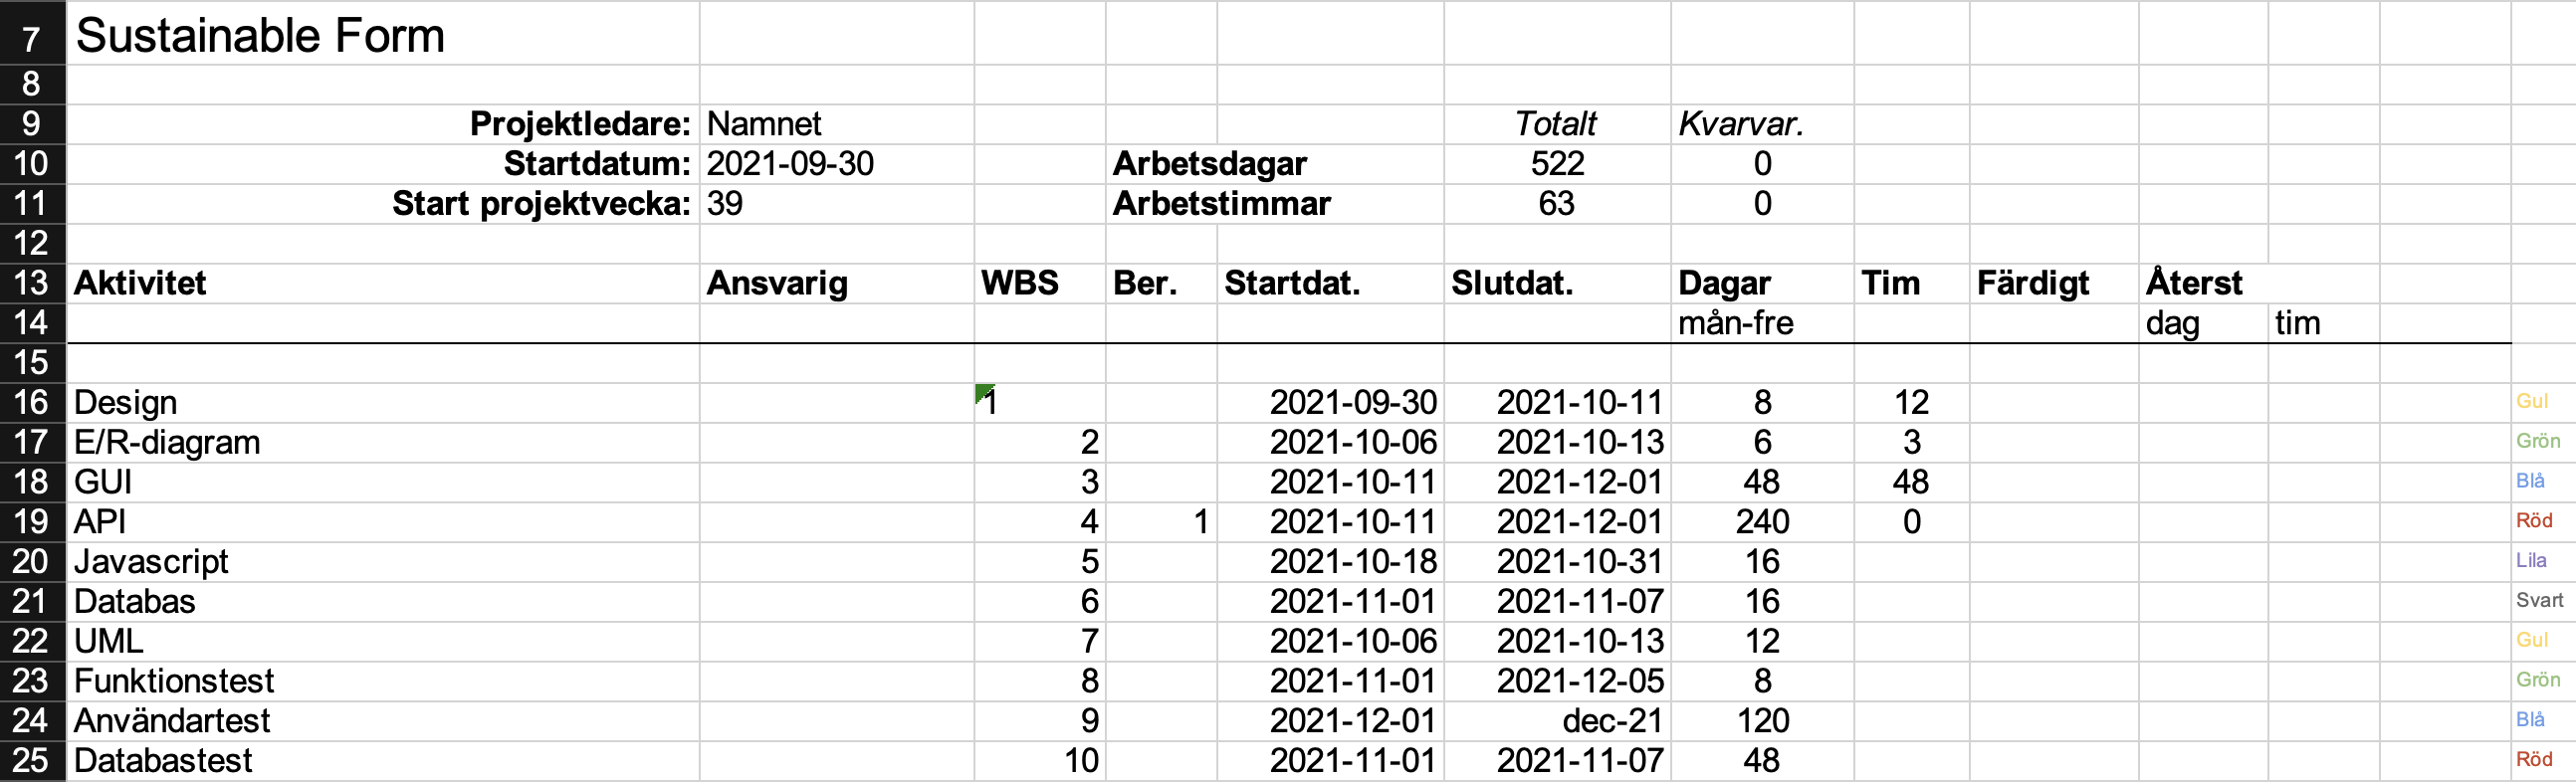
\includegraphics[width = 450px]{grant1.png}
    \label{fig:24}
\end{figure}

\begin{figure}[htp]
    \centering
    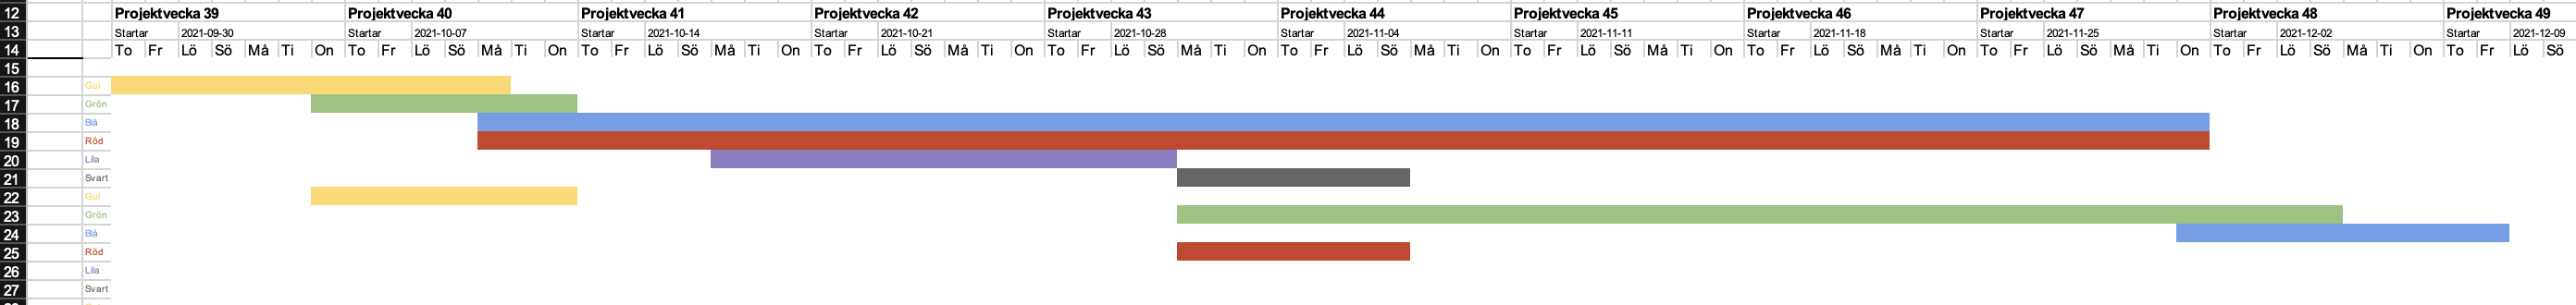
\includegraphics[width = 450px]{Grant2.png}
    \label{fig:24}
\end{figure}

\subsection{Team}
\subsection{Resultat}

\section{Utveckling och process}


\section{Referenser}

\section{Bilagor}
\subsection{Arbetsblad från motivering och process workshop}


\begin{figure}[htp]
    \centering
    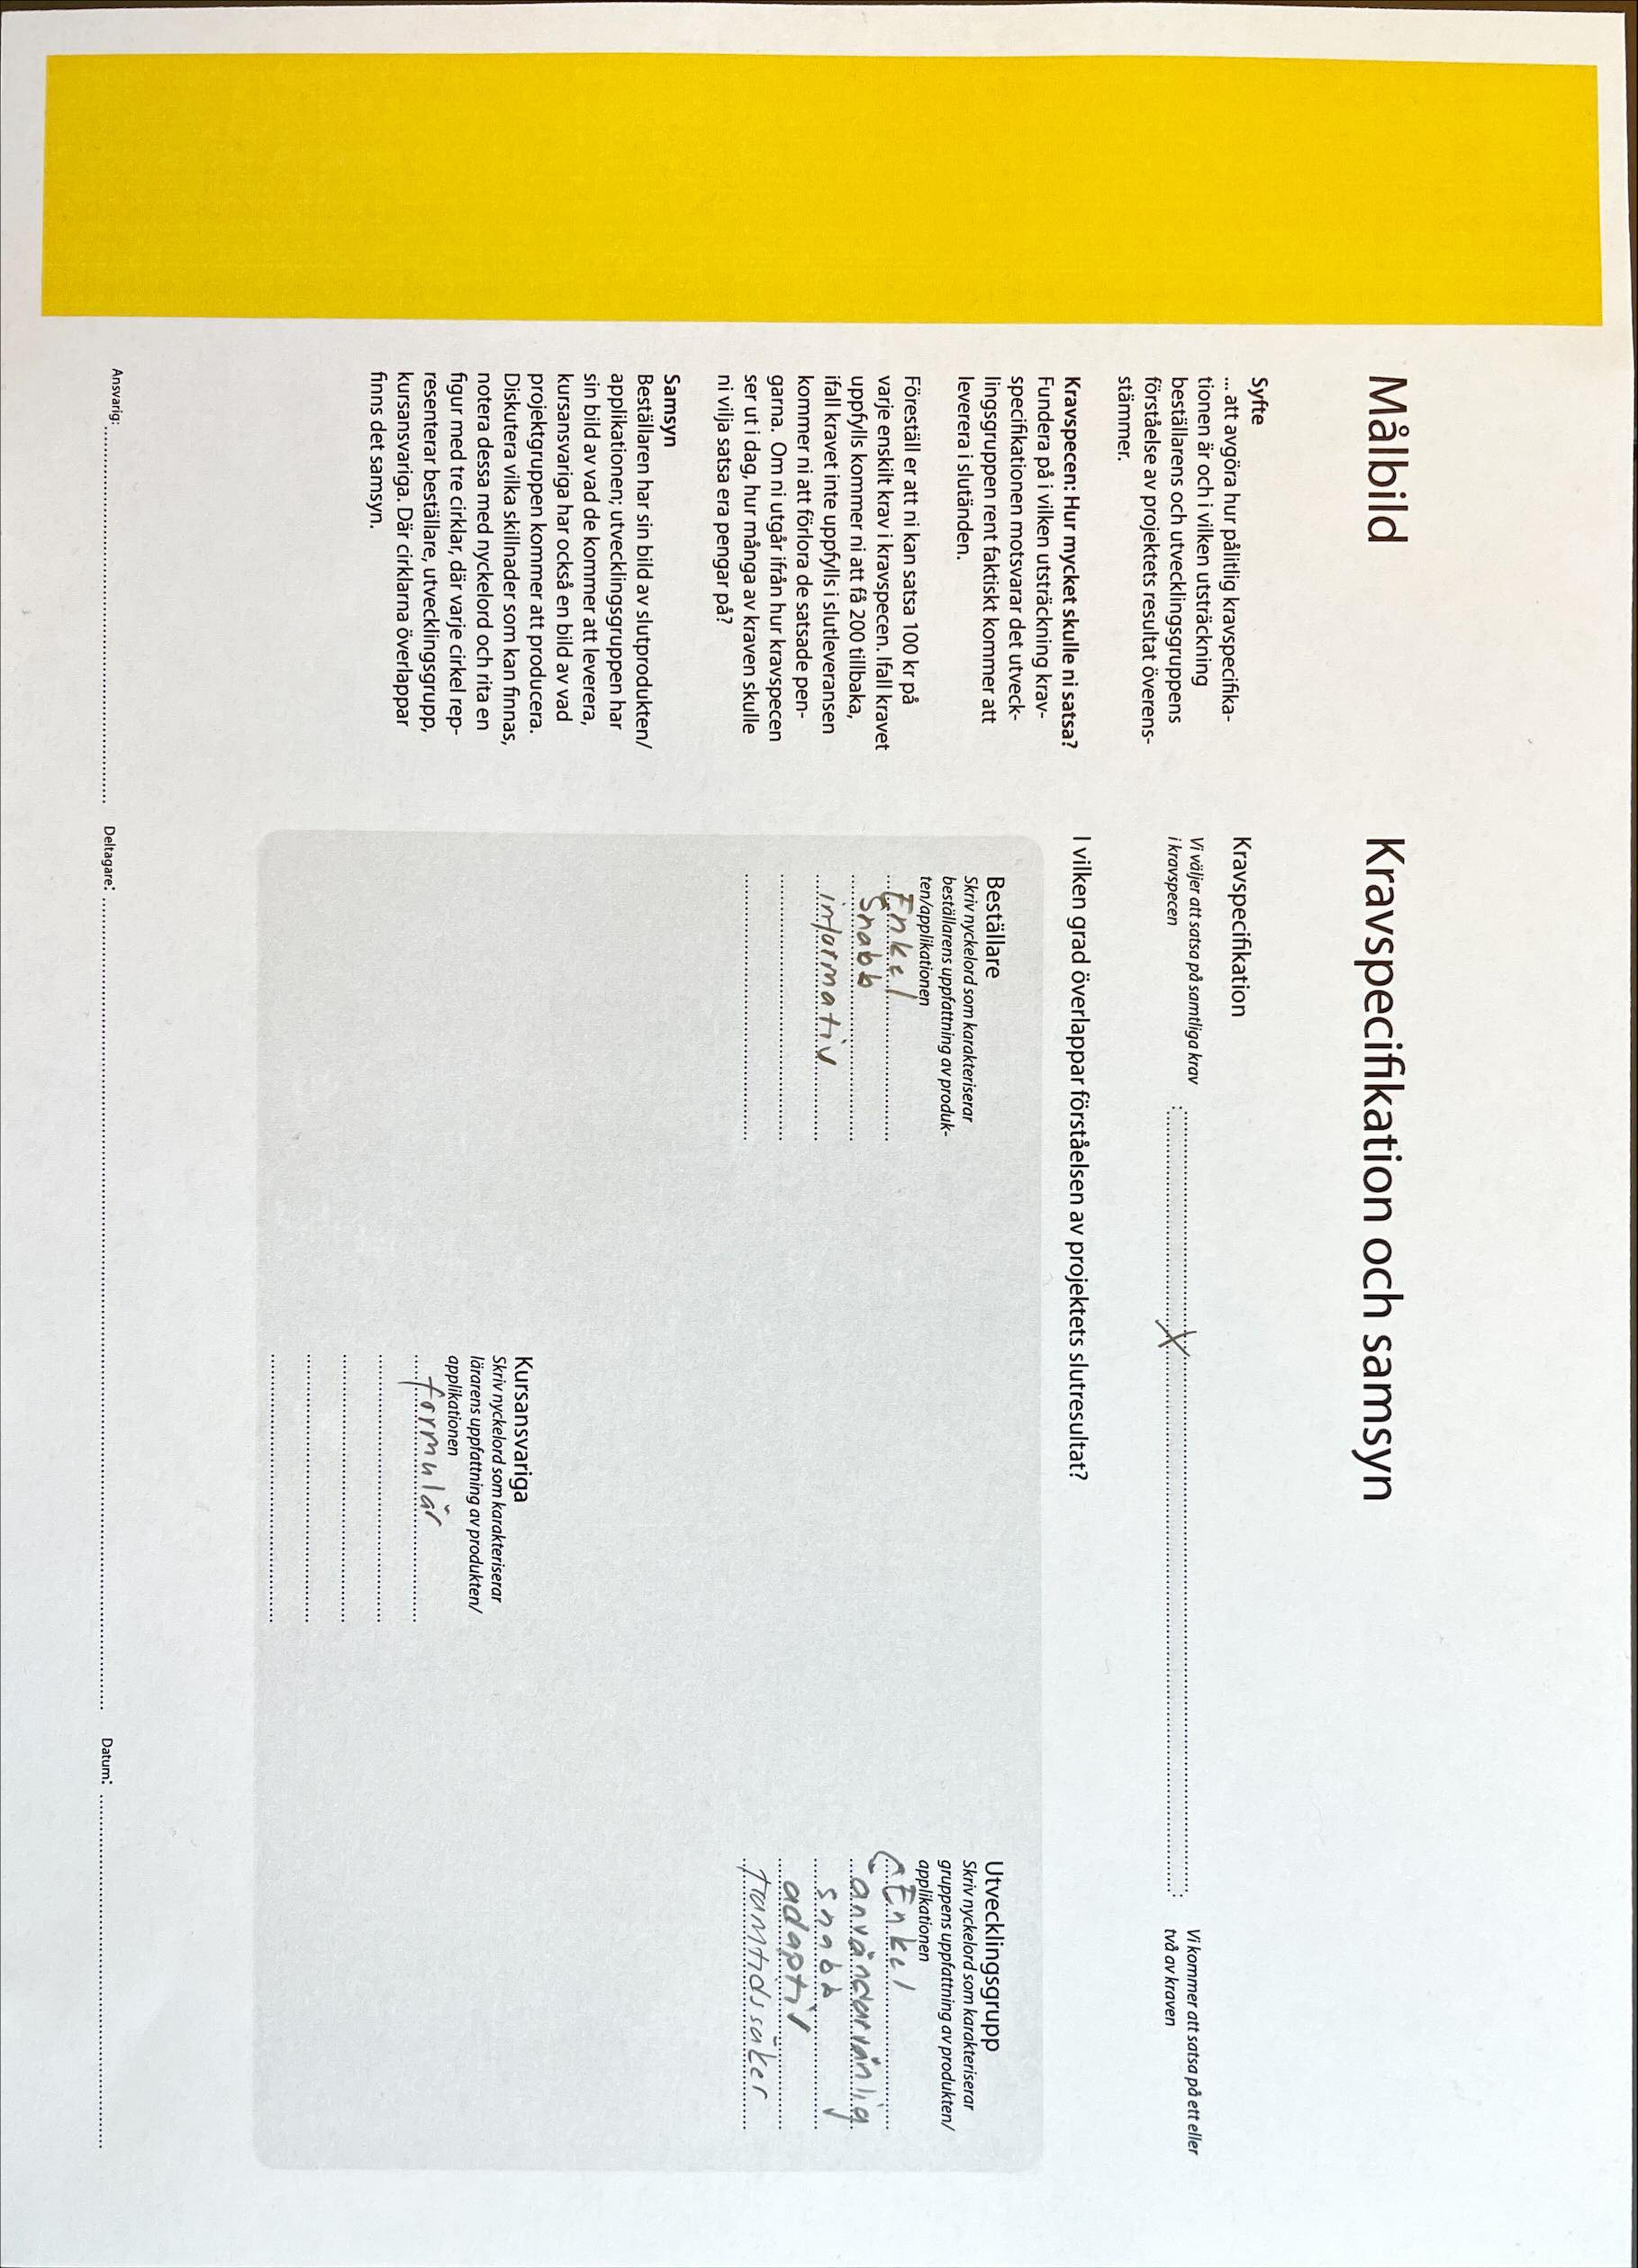
\includegraphics[width = 175px,angle=90]{KS.jpg}
    \label{fig:24}
\end{figure}

\begin{figure}[htp]
    \centering
    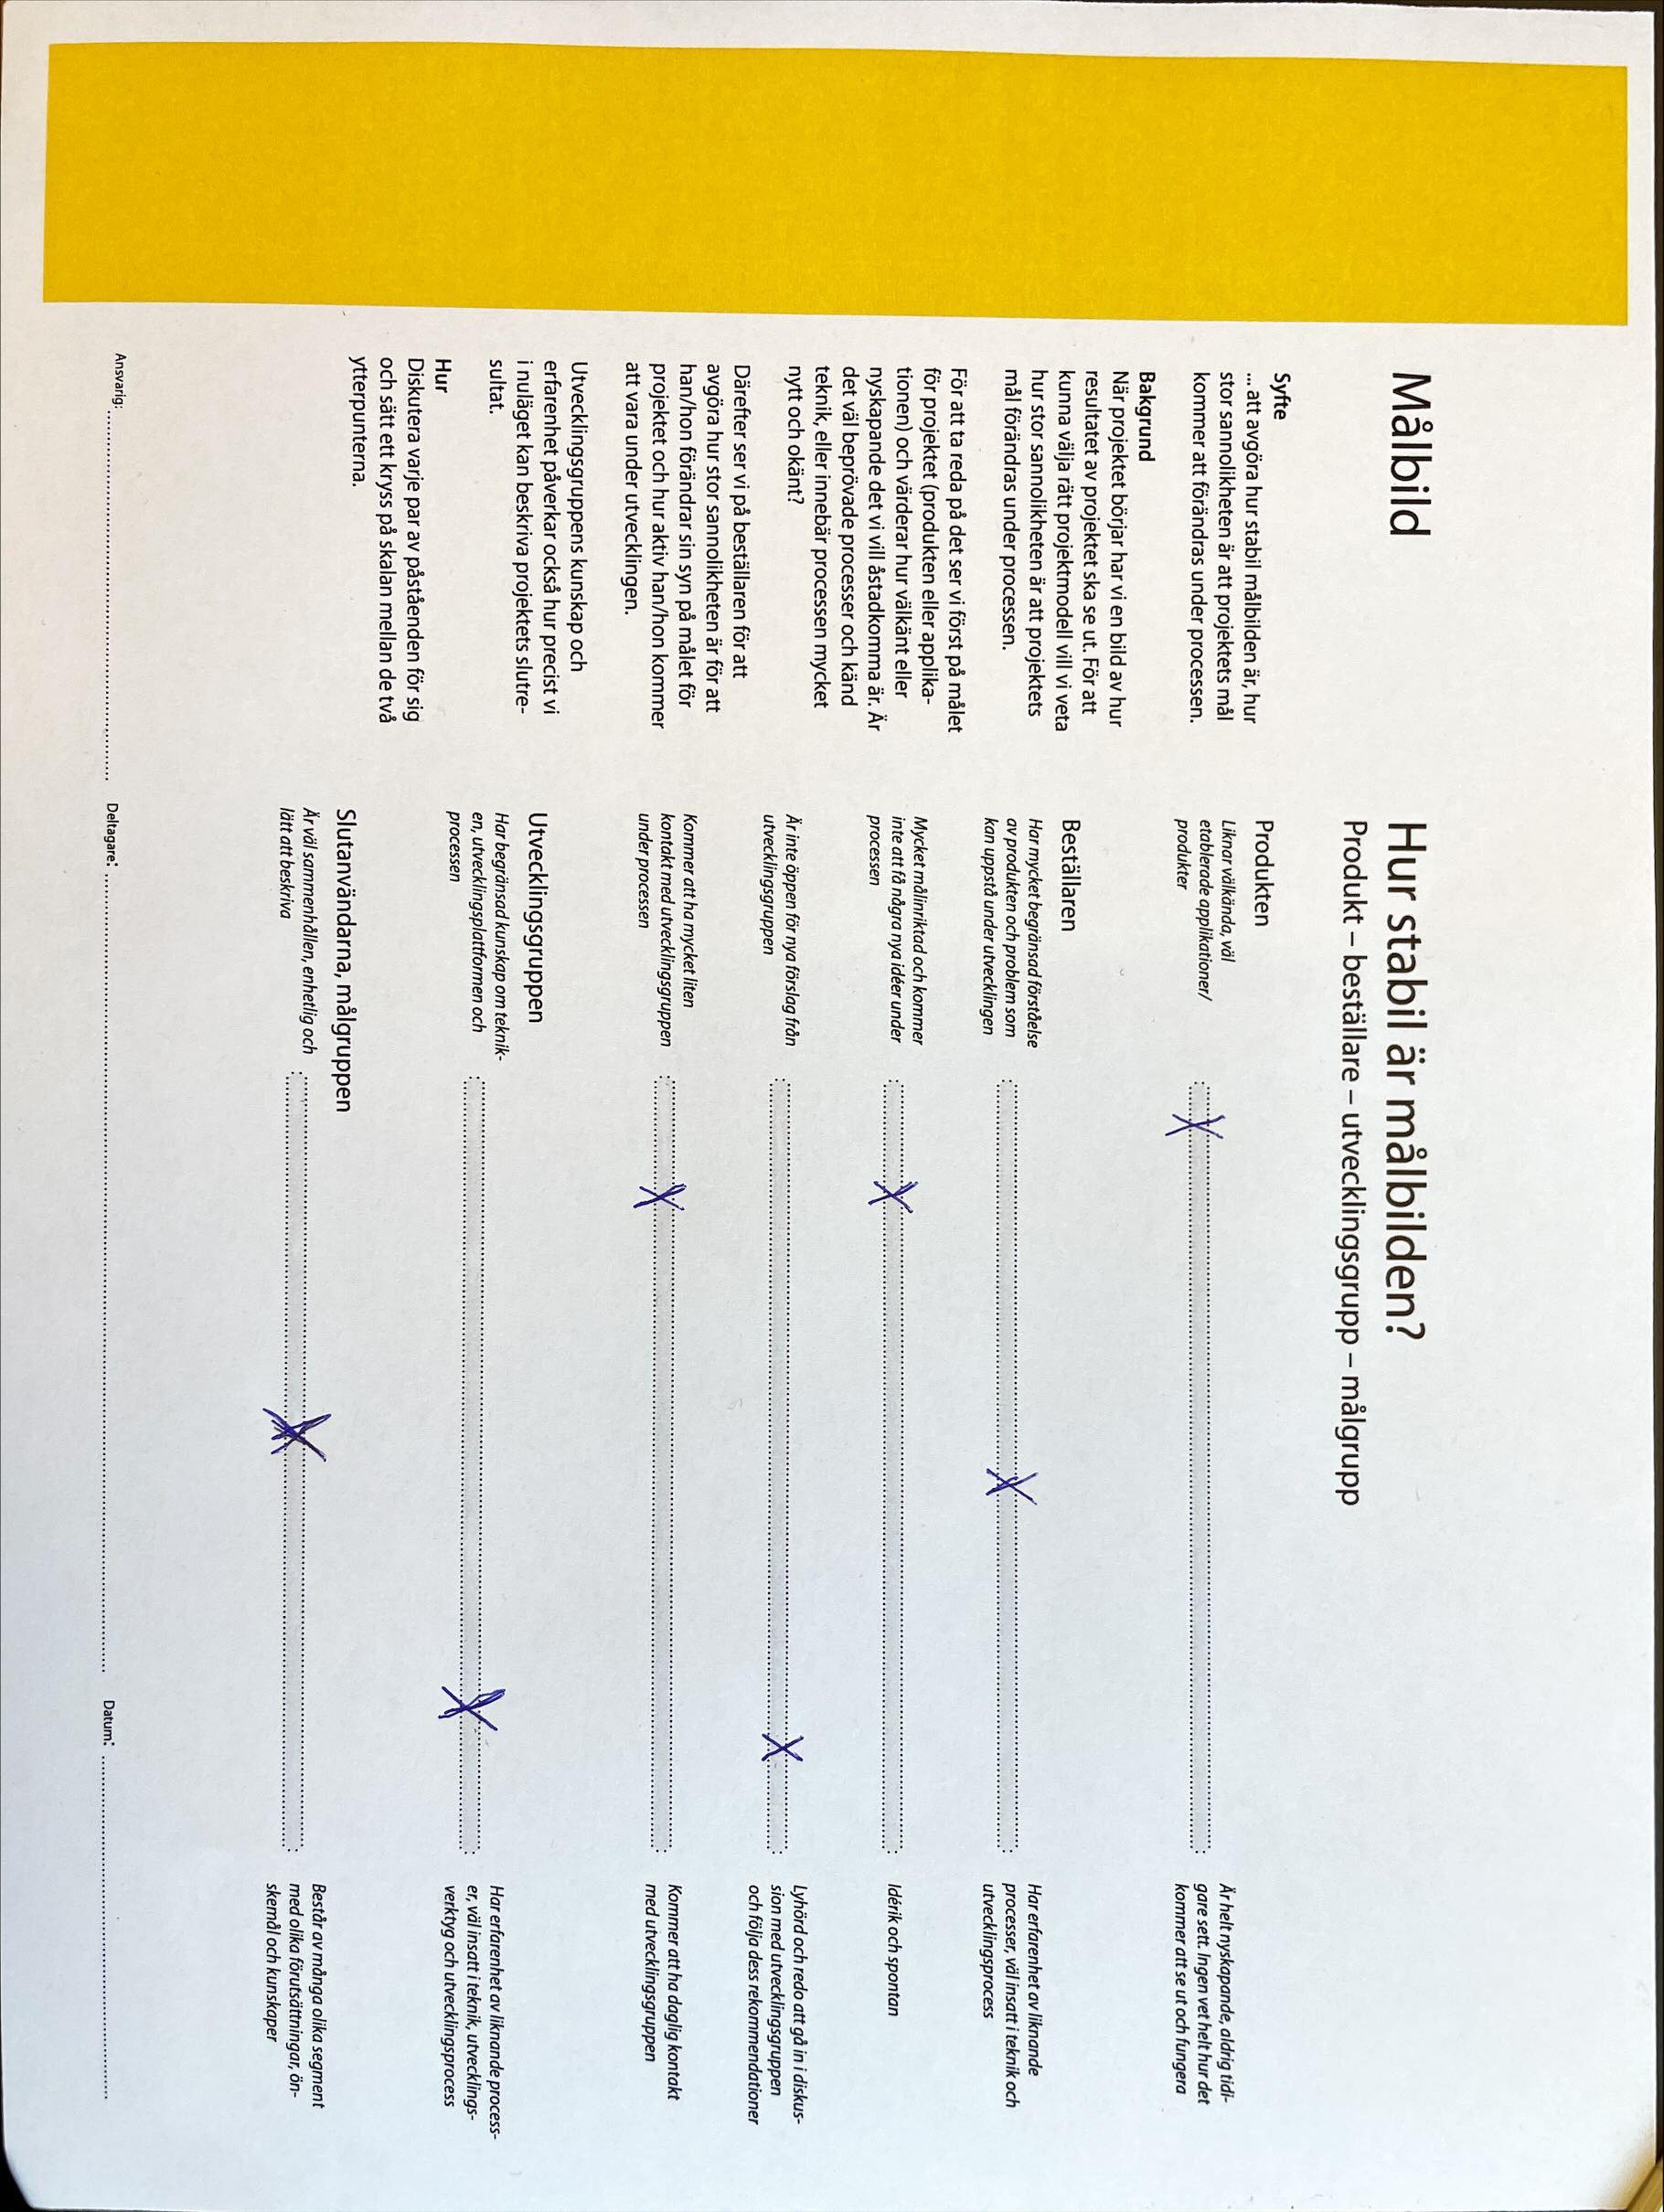
\includegraphics[width = 180px,angle=90]{SM.jpg}
    \label{fig:24}
\end{figure}

\begin{figure}[htp]
    \centering
    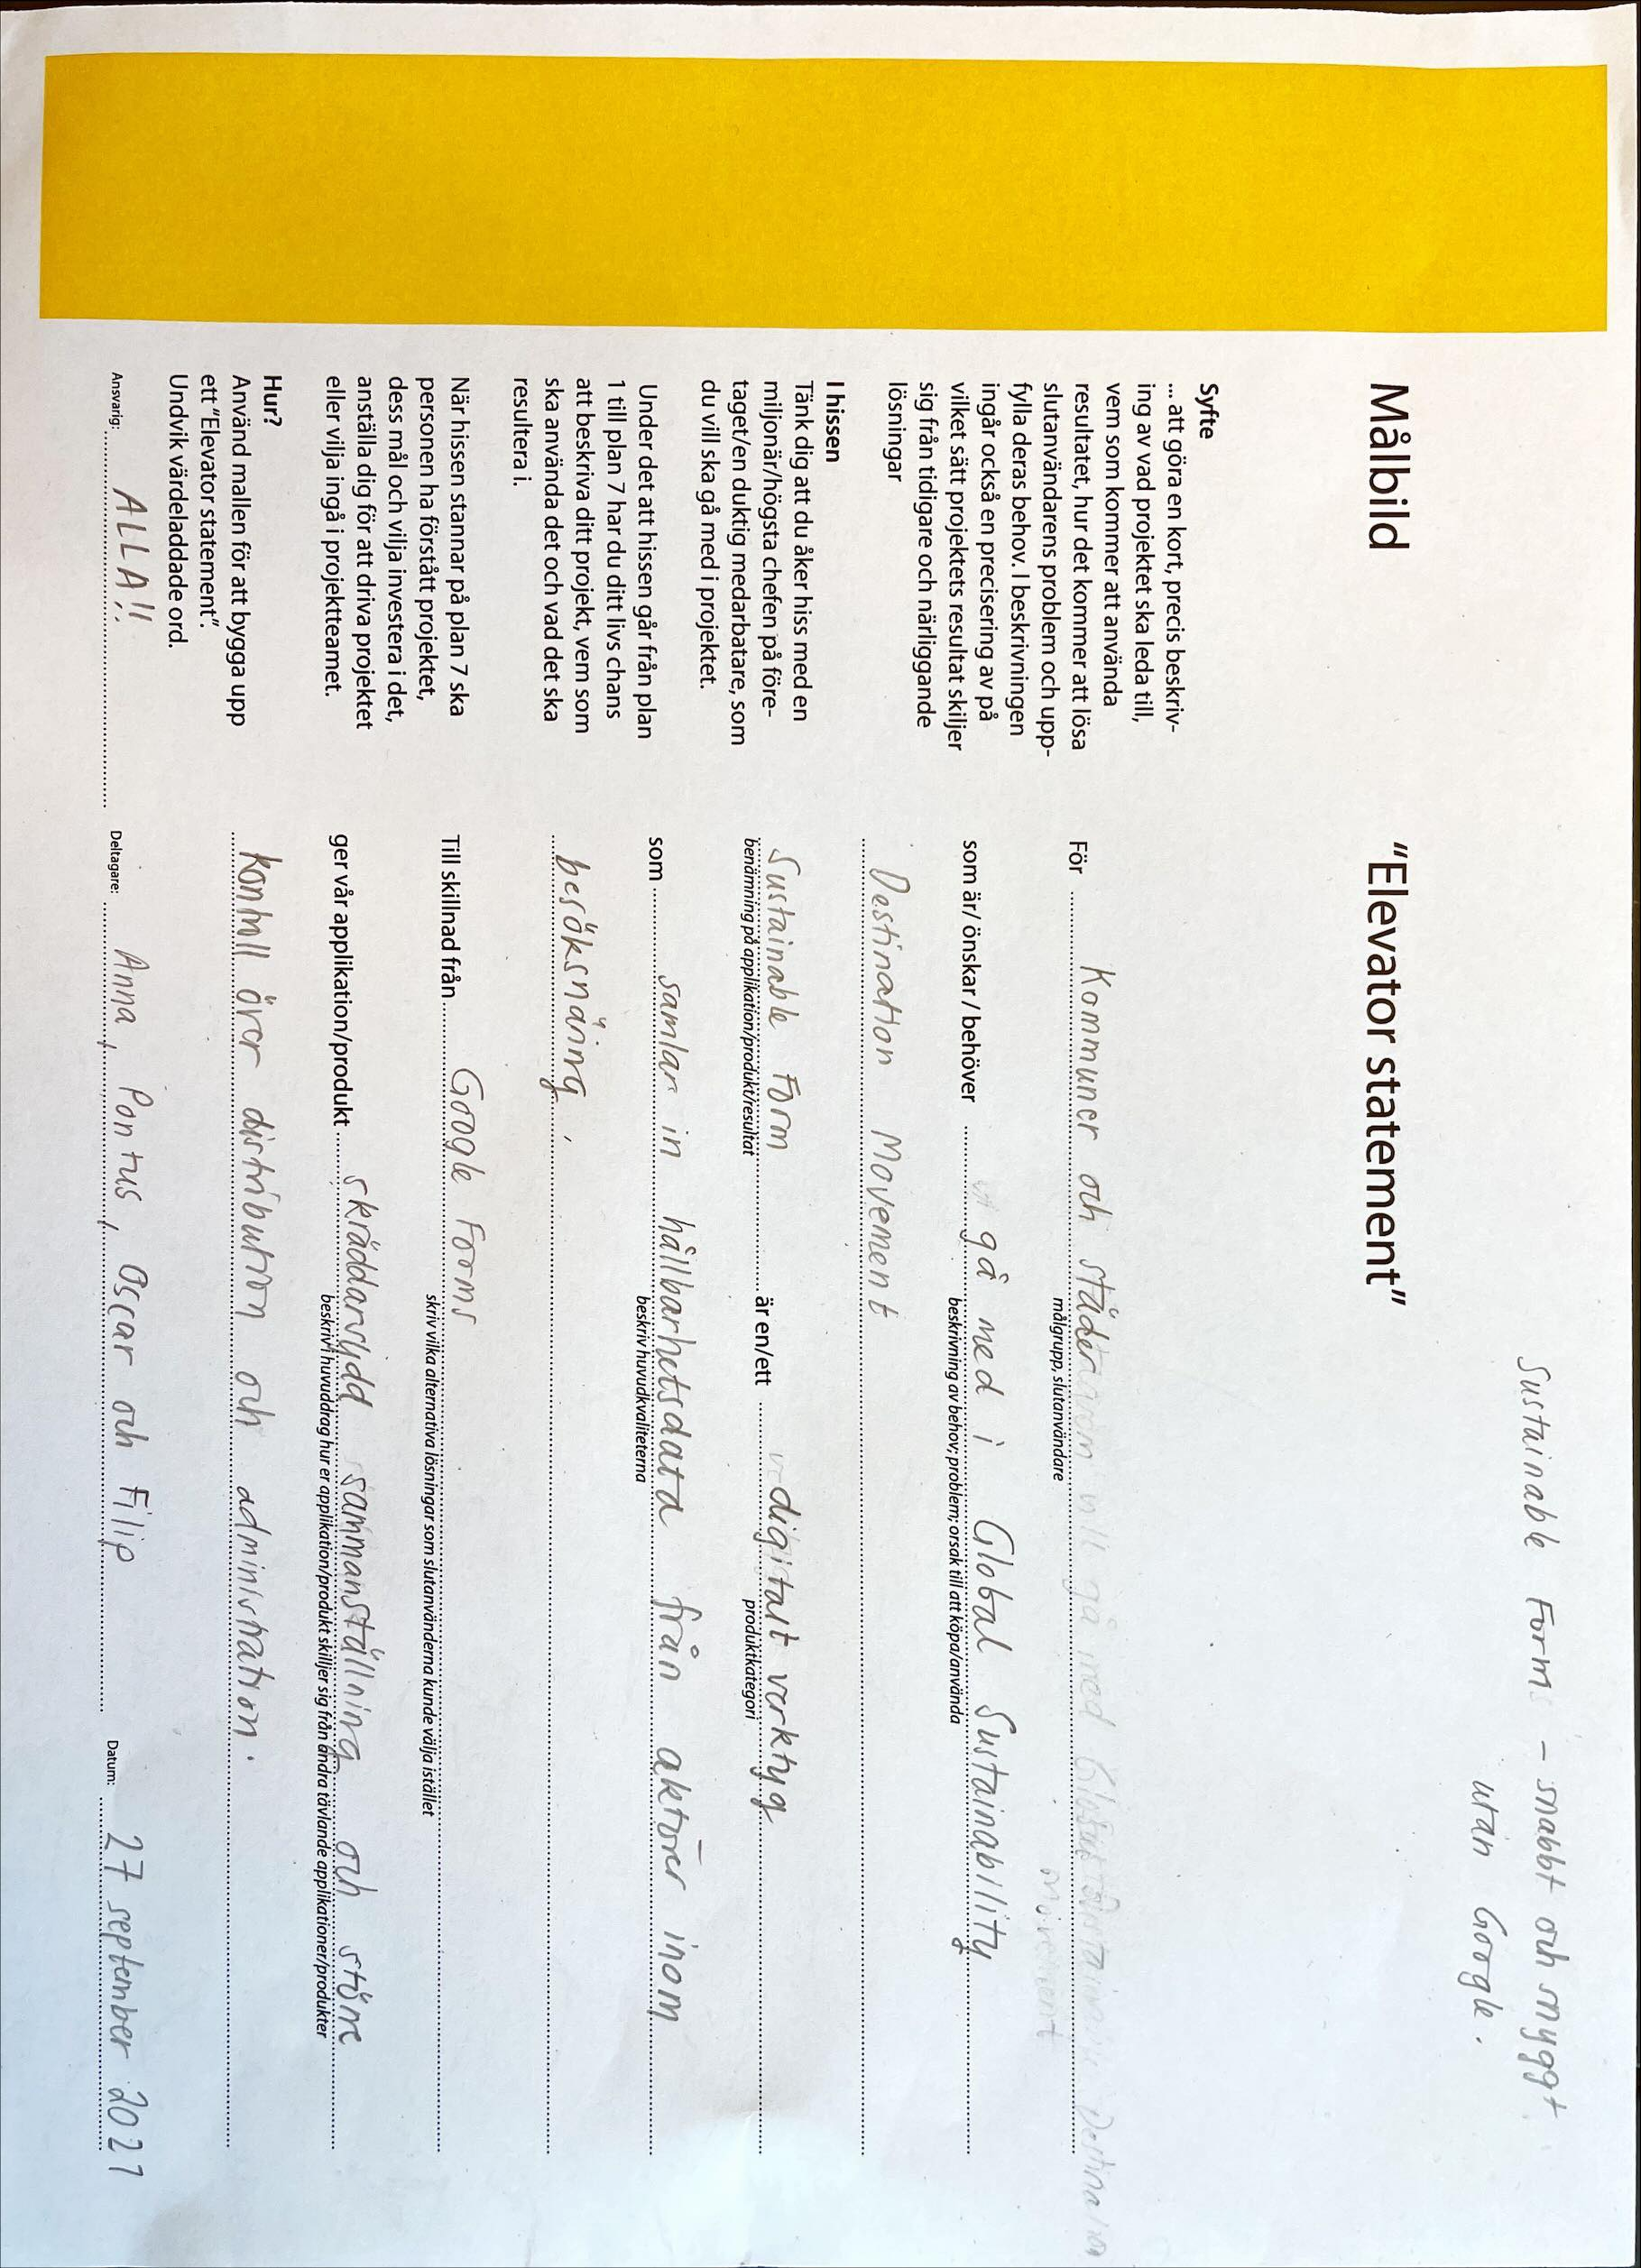
\includegraphics[width = 175px,angle=90]{Elev.jpg}
    \label{fig:24}
\end{figure}

\begin{figure}[htp]
    \centering
    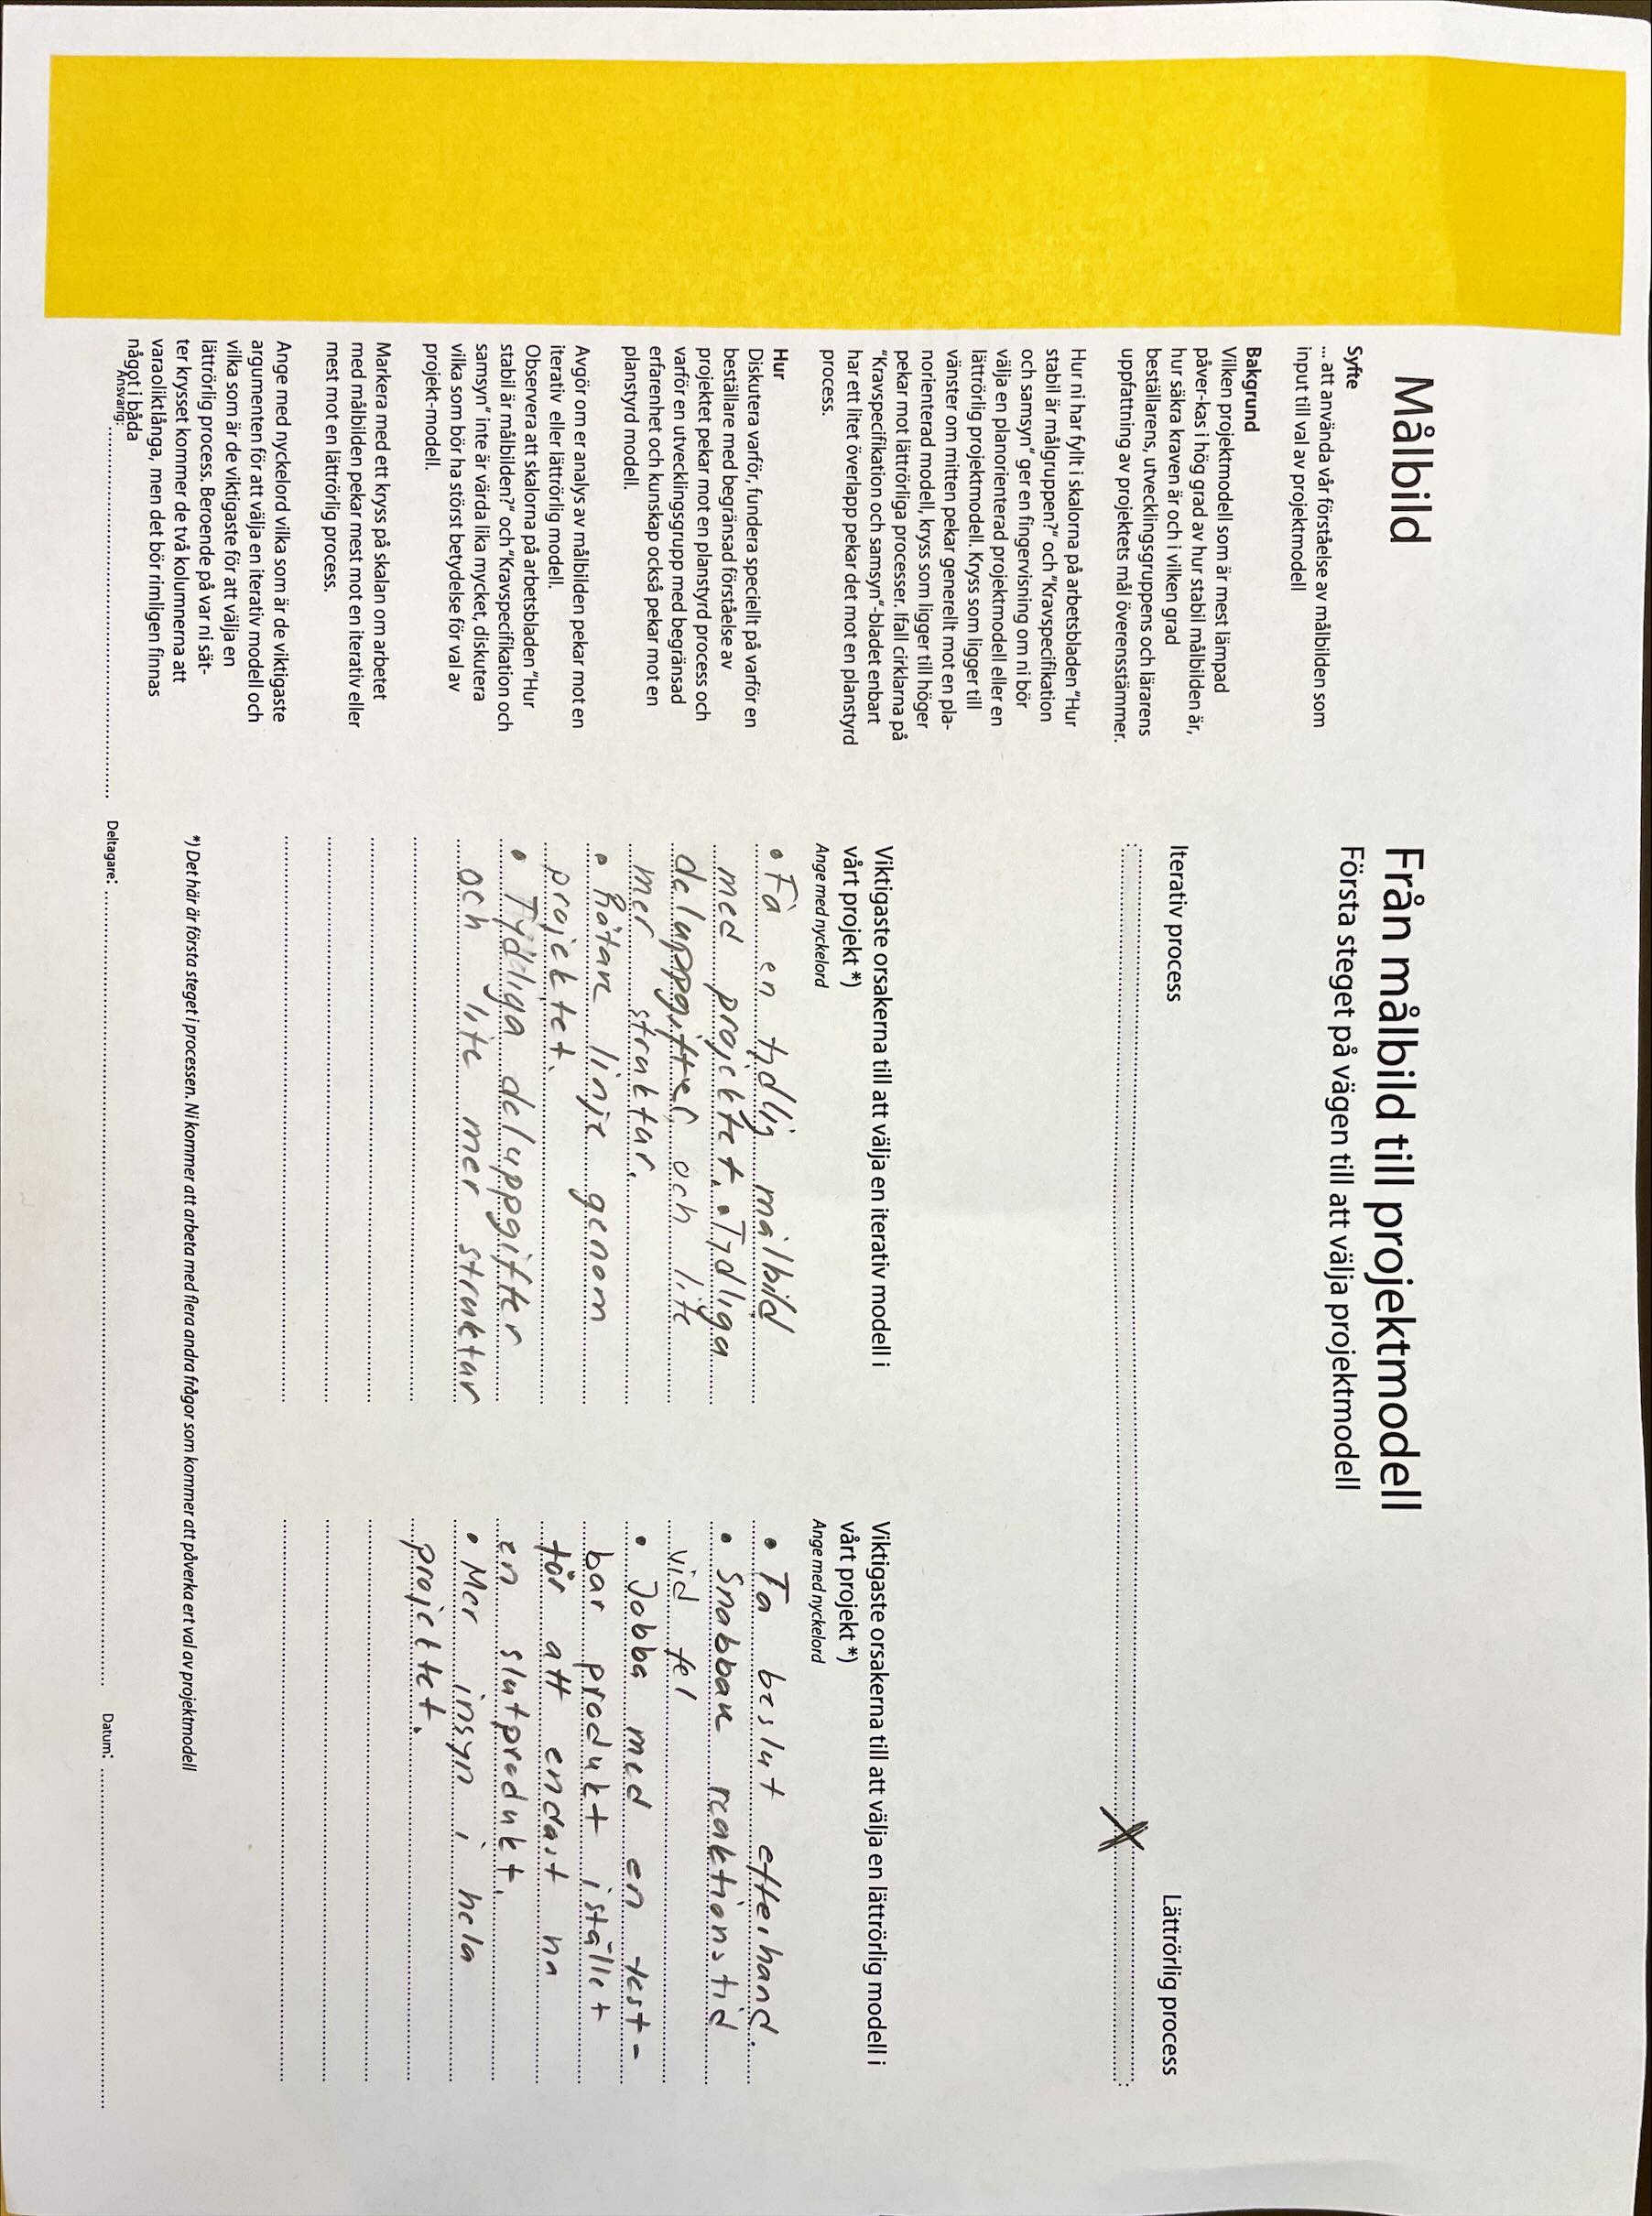
\includegraphics[width = 180px,angle=90]{MP.jpg}
    \label{fig:24}
\end{figure}





\bibliographystyle{alpha}


\end{document}